%---------------------------------------------------------------------
% Course 	: Introduction To web sciences
% Professor : Dr.Nelson
% Name   	: Babitha Bokka
% Assignment: 4
%---------------------------------------------------------------------
\documentclass[12pt]{article}
%--------------------------------------------------------------------
% packages required
%--------------------------------------------------------------------
\usepackage{graphicx}
\usepackage{listings}
\usepackage{hyperref}
\usepackage{caption}
\usepackage{color}
\usepackage{pdfpages}
\graphicspath{ {images/} }
%--------------------------------------------------------------------
% Start Margins
%--------------------------------------------------------------------
\addtolength{\oddsidemargin}{-.875in}
\addtolength{\evensidemargin}{-.875in}
\addtolength{\textwidth}{1.75in}
\addtolength{\topmargin}{-.885in}
\addtolength{\textheight}{1.95in}
%-------------------------------------------------------------------
% End Margins
%--------------------------------------------------------------------
\definecolor{codegreen}{rgb}{0,0.6,0}
\definecolor{codegray}{rgb}{0.5,0.5,0.5}
\definecolor{codepurple}{rgb}{0.58,0,0.82}
\definecolor{backcolour}{rgb}{0.95,0.95,0.92}
 
\lstdefinestyle{mystyle}{
    backgroundcolor=\color{backcolour},   
    commentstyle=\color{codegreen},
    keywordstyle=\color{magenta},
    numberstyle=\tiny\color{codegray},
    stringstyle=\color{codepurple},
    basicstyle=\footnotesize,
    breakatwhitespace=false,         
    breaklines=true,                 
    captionpos=b,                    
    keepspaces=true,                 
    numbers=left,                    
    numbersep=5pt,                  
    showspaces=false,                
    showstringspaces=false,
    showtabs=false,                  
    tabsize=2
}
 
\lstset{style=mystyle}

\begin{document}

%---------------------------------------------------------------------
%Making the title page
%---------------------------------------------------------------------
\begin{titlepage}
\title{INTRODUCTION TO WEB SCIENCES:\\*Assignment 4}
\author{Babitha Bokka}
\date{10 october 2014}
\maketitle
\end{titlepage}

%---------------------------------------------------------------------
%Table of contents
%---------------------------------------------------------------------
\tableofcontents
\newpage
%------------------------------------------------------------------
%Question 1
%------------------------------------------------------------------
\section{Question 1}
Choose 100 links from 1000 unique links and extract the outbound links from that page to other URIs.
%-----------------------Approach----------------------------------
\subsection{Approach}
To extract the outgoing links from the 100 URIs extractHyperLinks.py is loaded with the 1000 unique URIs. The LIMIT value in the program selects only 100 URIs, these are URIs which can establish the connection and has no exceptions.
\subsection{Description of extractHyperLinks.py}
\begin{enumerate}
	\item Open the A2FinalOutput.txt.
	\item Read each URL and extract the outgoing links.
	\item Out of 1000 Unique URIs the Program will extract 100 working URIs and get the outgoing links from each URI.
	\item Create a md5 file and write all the links to the ``.link'' file at the same time a log file (md5Links.txt) is generated which has the md5 and URL.	
	\item All the file are saved in A4/Q1/links.	
\end{enumerate}
\newpage
%-----------------------Source Code-------------------------------
\subsection{Source Code}
\subsubsection{extractHyperLinks.py}
\lstinputlisting[breaklines=True,language=Python]{../Q1/extractHyperLinks.py}
\newpage
%-----------------------Input Section----------------------------
\subsection{Input Files}
\subsubsection{A2FinalOutput.txt}
\lstinputlisting[breaklines=True]{../Q1/uniqueForDoc.txt}
\newpage
%-----------------------Output Section---------------------------
\subsection{Output Files}
Aim : To generate the 100 ``.link'' files which have the outbound links from that page to other URIs.The files are saved in A4/Q1/links.
\subsubsection{md5Links.txt}
The file acts as a logfile to keep track of URI and corresponding md5 file.
\lstinputlisting[breaklines=True]{../Q1/md5uriFordoc.txt}

\subsubsection{a524329028e8dcfc4879b4b453c1040a.link}
A sample ``.link'' file having the outgoing links.
\lstinputlisting[breaklines=True]{../Q1/sampleContentOutputFile.txt}
\newpage
%-----------------------End Question 1----------------------------

%------------------------------------------------------------------
%Question 2
%------------------------------------------------------------------
\section{Question 2}
Generate a single DOT file for 100 links. 
%-----------------------Approach----------------------------------
\subsection{Description of createDotFile.py}
\begin{enumerate}
	\item Open the md5Links.txt, extract the url and md5.
	\item Using glob to find the respective folder.	
	\item Check whether md5 of the current URL and the file name in the folder are matching if, they match then open the file and append the links inside each file to the URL
	\item Write all the URL and respective links to ``mapping.dot'' file.	
\end{enumerate}

\newpage
%-----------------------Source Code-------------------------------
\subsection{Source Code}
\subsubsection{createDotFile.py}
\lstinputlisting[breaklines=True,language=Python]{../Q2/createDotFile.py}
\newpage
%-----------------------Input Section-----------------------------
\subsection{Input Files}
\subsubsection{md5Links.txt}
\lstinputlisting[breaklines=True]{../Q2/md5uriFordoc.txt}
\newpage
%-----------------------Output Section----------------------------
\subsection{Output Files}
\subsubsection{mapping.txt}
\lstinputlisting[breaklines=True]{../Q2/mappingforDoc.txt}
\newpage
%-----------------------End Question 1----------------------------

%------------------------------------------------------------------
%Question 3
%------------------------------------------------------------------
\section{Question 3}
Download and install Gephi then load the dot file to visualize the graph.
%-----------------------Approach----------------------------------
\subsection{Approach}
Downloaded gephi and loaded the mapping.dot file into the software. In order to get more insight of the visualization layouts Fruchterman, Reingold and Yifan  Hu and Yifan Hu Proportional are used. Run the layouts couple of time to get more insight and export them to a pdf or png format.
%-----------------------Source Code-------------------------------
\subsection{Input Files}
The input is the output of the Question 2.
\subsubsection{mapping.txt}
\lstinputlisting[breaklines=True]{../Q3/mappingforDoc.txt}
\newpage
%-----------------------Output Section----------------------------

\subsection{Visualization with labels}
The below graph depicts that there are not much connected components very few of the clusters are connected and few of them does not have outgoing links. \\*

The second figure shows you how the nodes and edges are connected and it clearly depicts whether the clusters are connected or not connected when compared to the visualization with labels. A clear insight can be obtained from connected.pdf by enlarging.
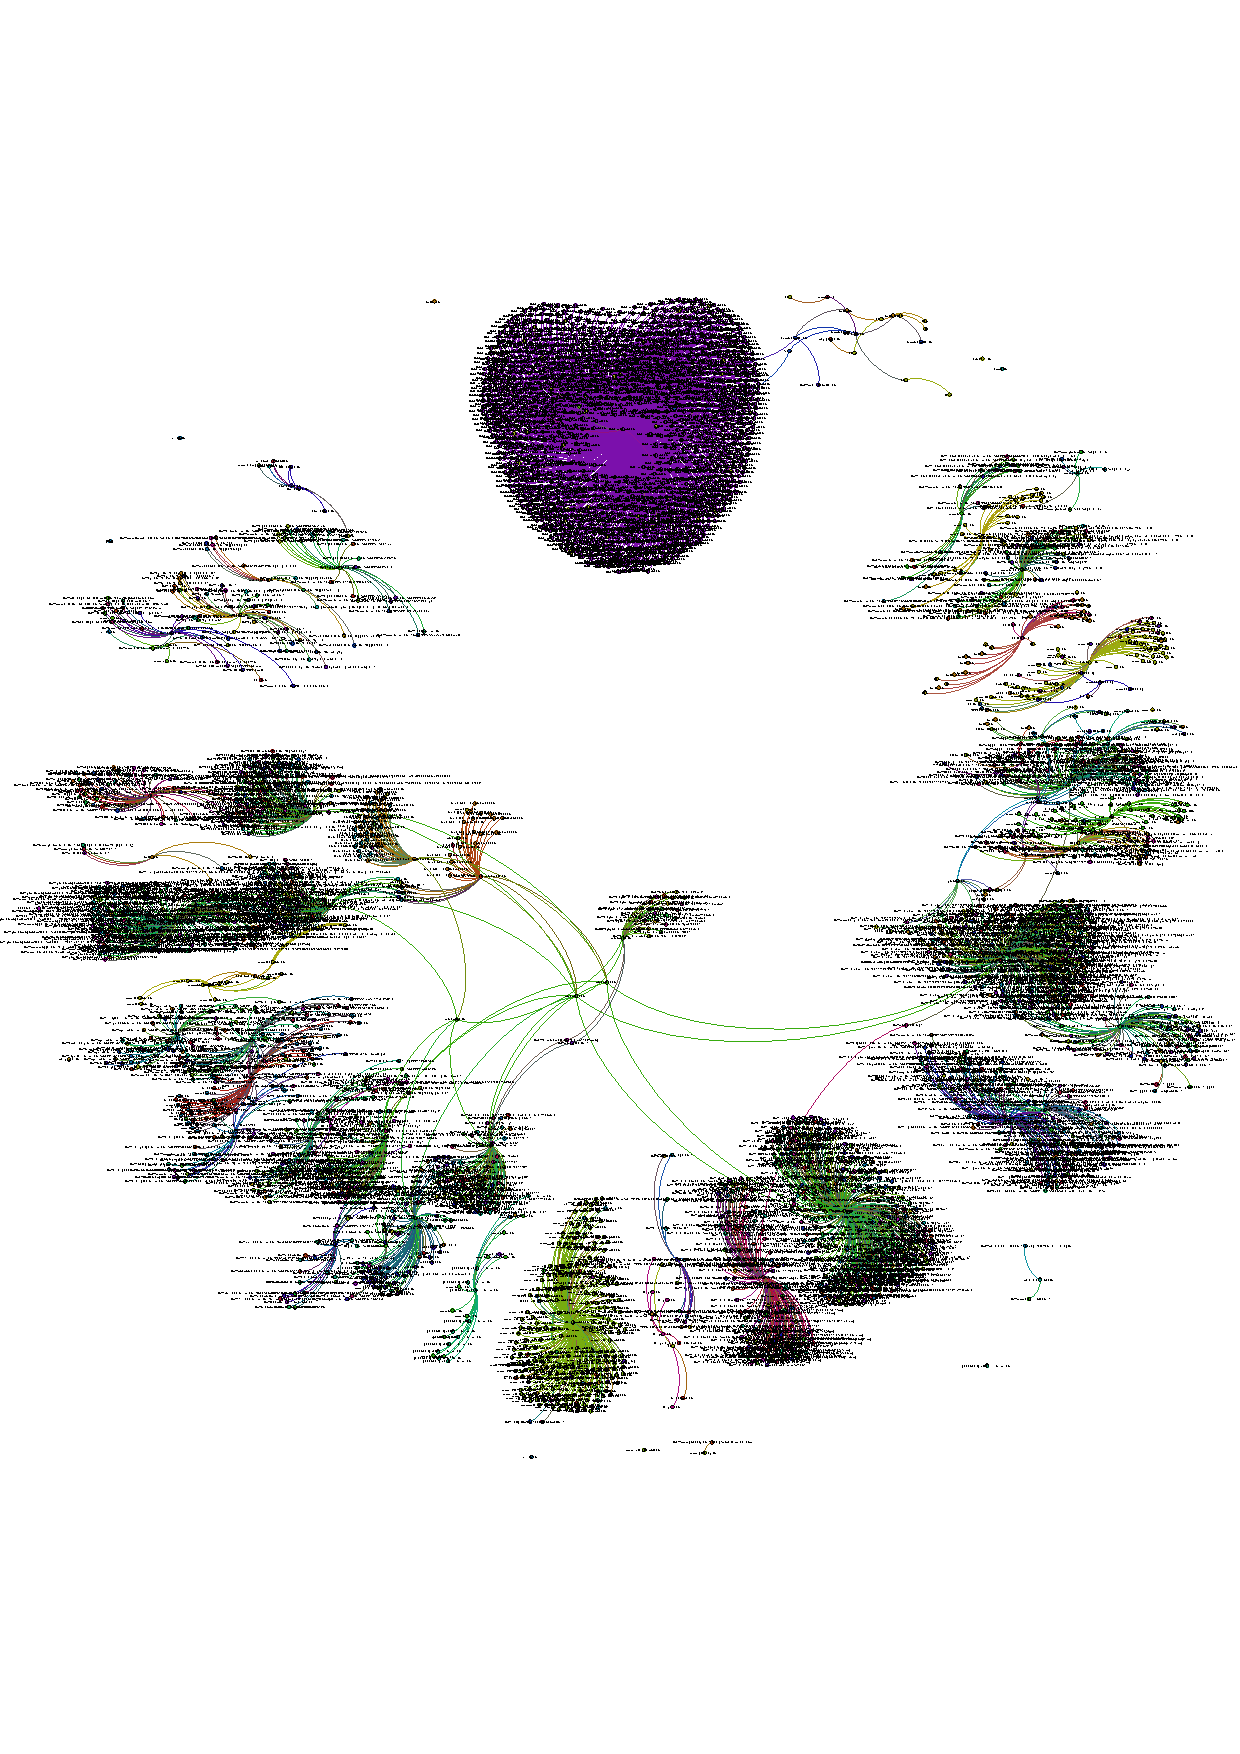
\includepdf[pages={1}]{../Q3/withLabels.pdf}
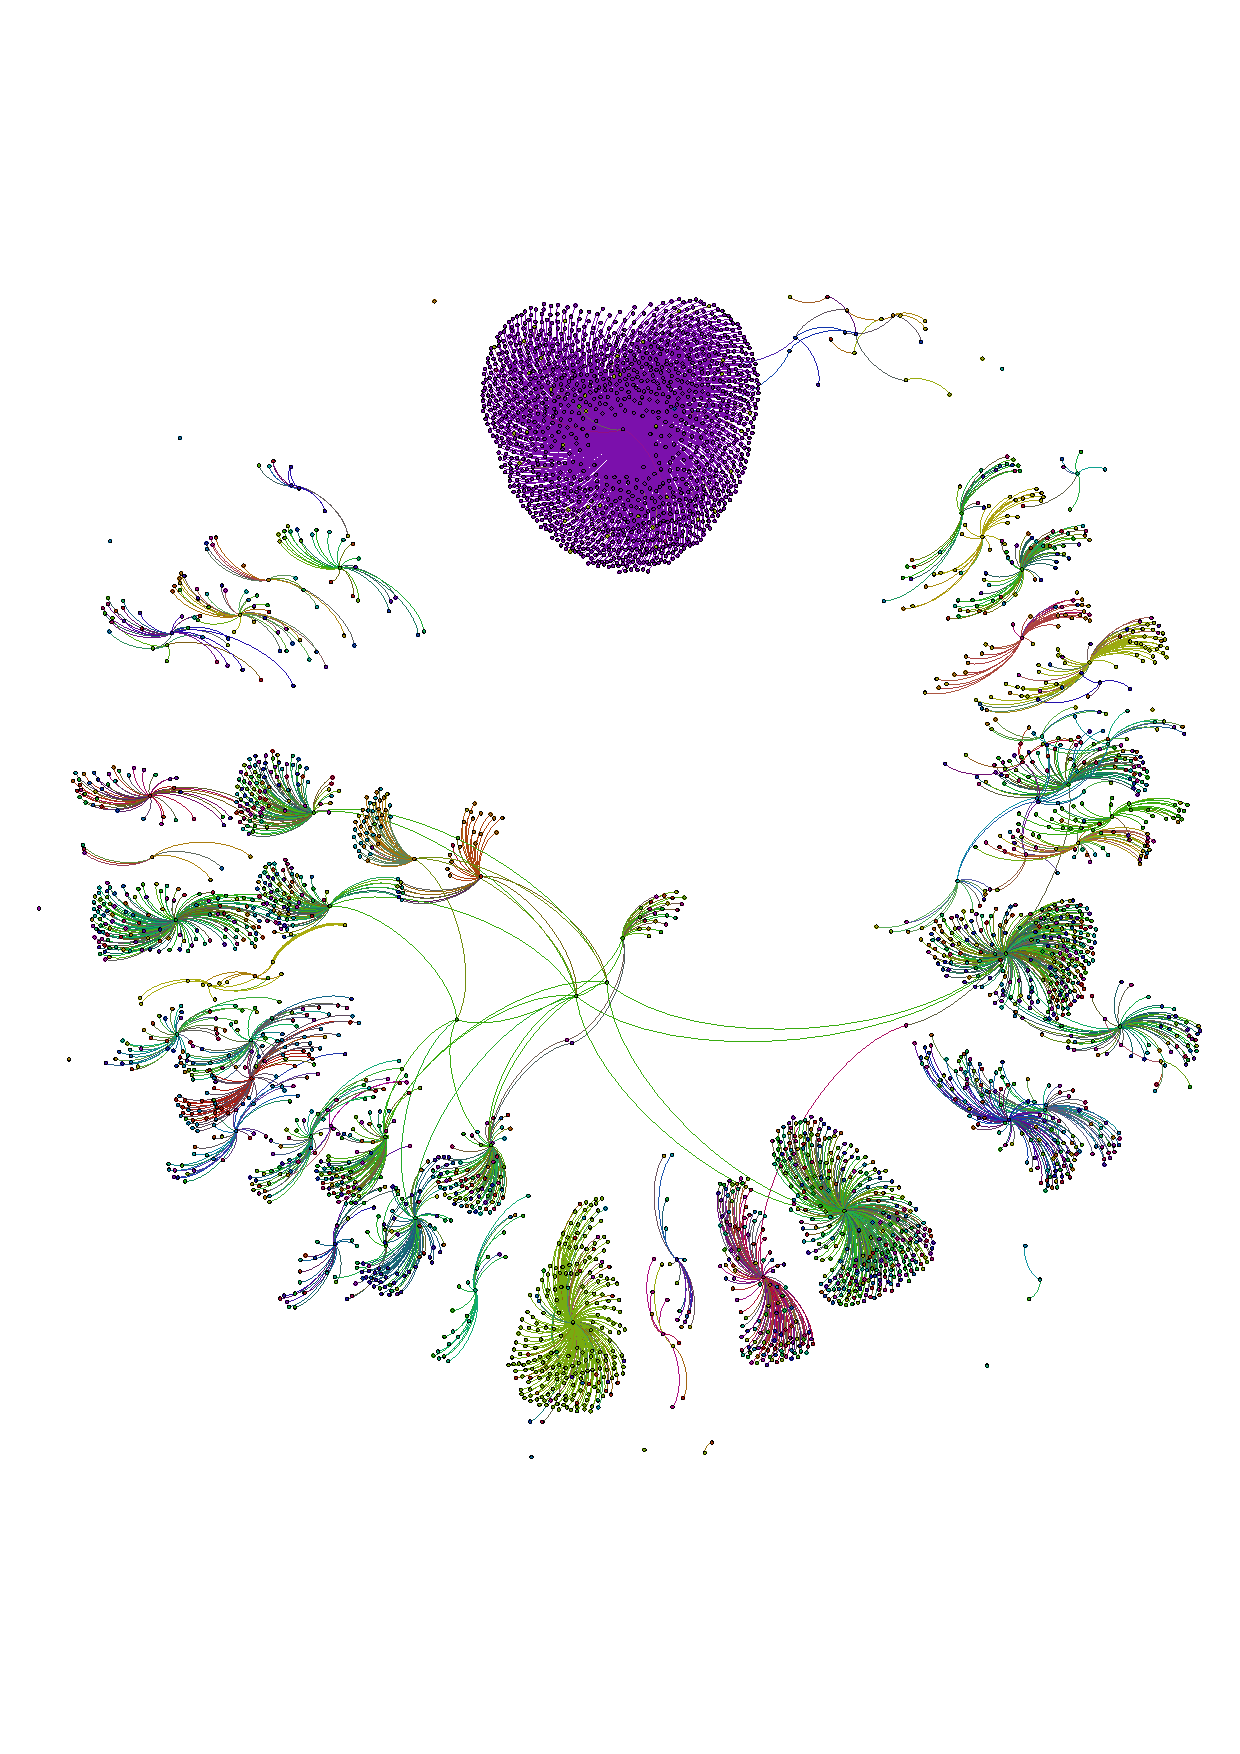
\includepdf[pages={1}]{../Q3/withOutLabels.pdf}
\newpage

\subsubsection{Hits}
\begin{figure}[h!]
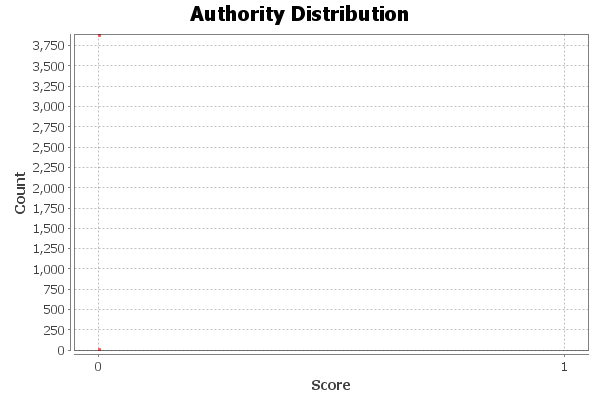
\includegraphics[scale=0.7]{../Q3/hits/authorities}
\caption{Authorities}
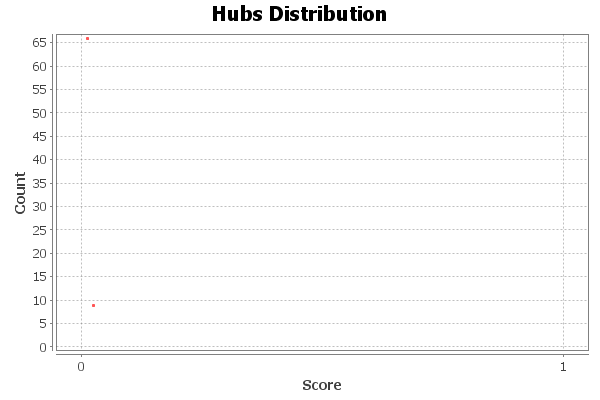
\includegraphics[scale=0.7]{../Q3/hits/hubs}
\caption{Hubs}
\end{figure}
\newpage

\subsubsection{PageRank}
Epsilon = 0.001\\*
Probability = 0.85
\begin{figure}[h!]
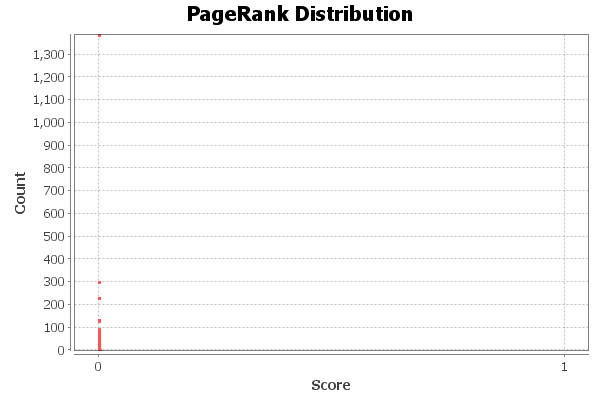
\includegraphics[scale=0.7]{../Q3/pagerank/pageranks}
\centering
\caption{pagerank of links}
\end{figure}
\newpage

\subsubsection{Average}
Average Degree: 0.997
\begin{figure}[!ht]
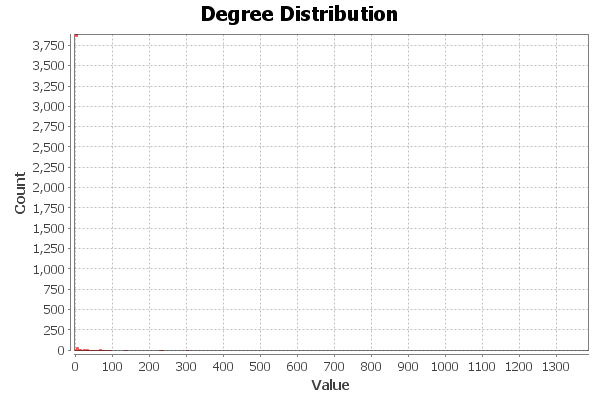
\includegraphics[scale=0.7]{../Q3/average/degree-distribution}
\centering
\caption{Average degree-distribution}
\end{figure}

\begin{figure}[!ht]
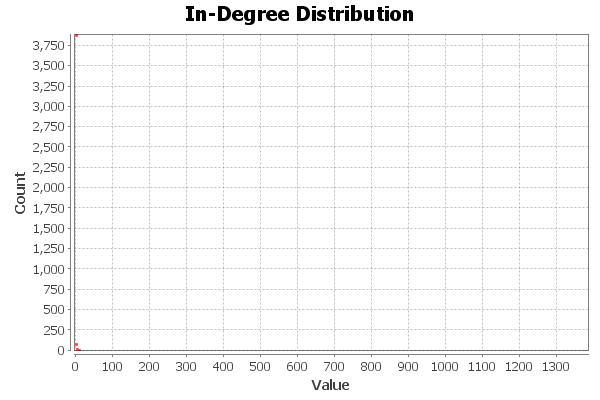
\includegraphics[scale=0.7]{../Q3/average/indegree-distribution}
\centering
\caption{Average indegree-distribution}
\end{figure}
\newpage
\begin{figure}[!ht]
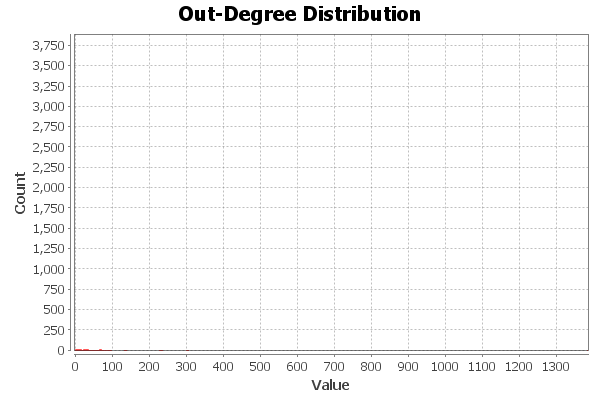
\includegraphics[scale=0.7]{../Q3/average/outdegree-distribution}
\centering
\caption{average outdegree-distribution}
\end{figure}
\newpage

\subsubsection{Network Diameter}
Diameter: 1\\*
Radius: 0\\*
Average Path length: 1.0\\*
Number of shortest paths: 3969
\begin{figure}[!ht]
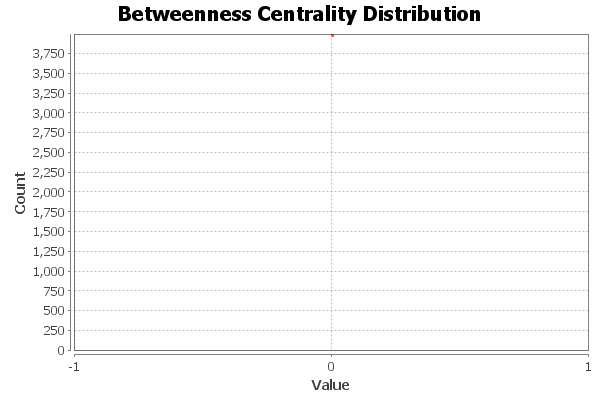
\includegraphics[scale=0.7]{../Q3/network/BetweennessCentralityDistribution}
\centering
\caption{Betweeness}
\end{figure}

\begin{figure}[!ht]
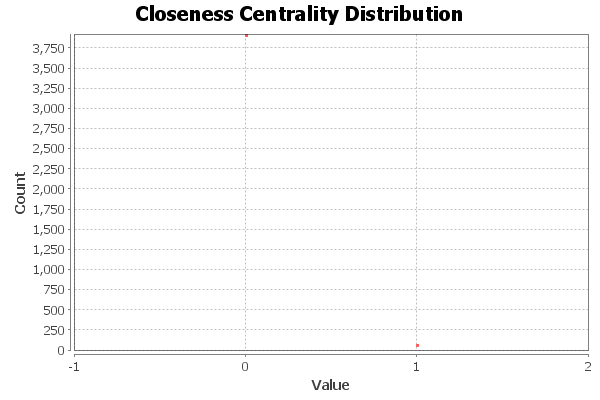
\includegraphics[scale=0.7]{../Q3/network/ClosenessCentralityDistribution}
\centering
\caption{Closeness}
\end{figure}
\newpage
\begin{figure}[!ht]
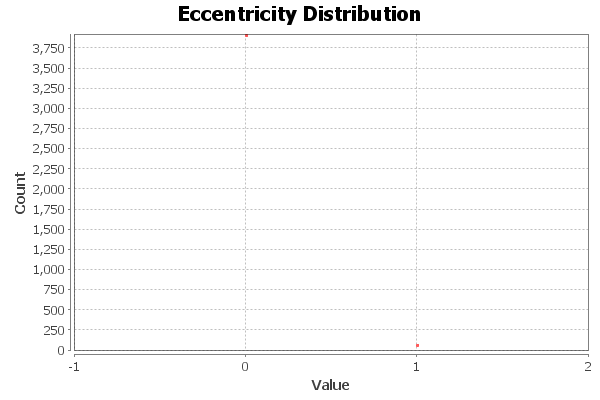
\includegraphics[scale=0.7]{../Q3/network/EccentricityDistribution}
\centering
\caption{EccentricityDistribution}
\end{figure}
\newpage

\subsubsection{Connected Components}
Number of Weakly Connected Components: 58\\*
Number of Stronlgy Connected Components: 3990
\begin{figure}[h!]
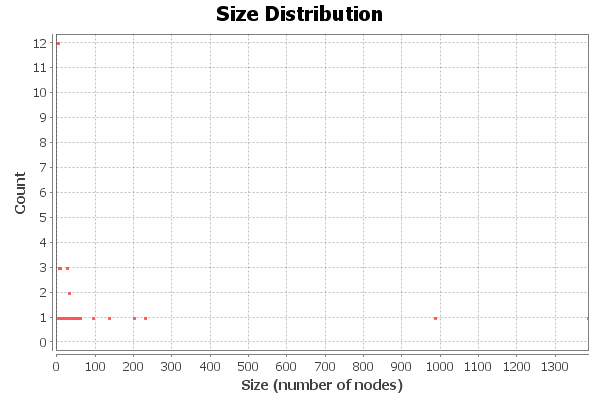
\includegraphics[scale=0.7]{../Q3/connected/cc-size-distribution}
\centering
\caption{Graph Connected Components}
\end{figure}
\newpage
%-----------------------End Question 3----------------------------

%------------------------------------------------------------------
%Bibilography
%------------------------------------------------------------------
\bibliographystyle{plain}
\bibliography{A4_report}
\cite{*}
\end{document}